%%% License: Creative Commons Attribution Share Alike 4.0 (see https://creativecommons.org/licenses/by-sa/4.0/)


%%%%%%%%%%%%%%%%%%%%%%%%%%%%%%%%%%%%%%%%%

%----------------------------------------------------------------------------------------
%	PACKAGES AND OTHER DOCUMENT CONFIGURATIONS
%----------------------------------------------------------------------------------------

\documentclass{article}

\usepackage{amssymb}
\usepackage{enumerate}
\usepackage[usenames,dvipsnames]{color}
\usepackage{fancyhdr} % Required for custom headers
\usepackage{lastpage} % Required to determine the last page for the footer
\usepackage{extramarks} % Required for headers and footers
\usepackage[usenames,dvipsnames]{color} % Required for custom colors
\usepackage{graphicx} % Required to insert images
\usepackage{listings} % Required for insertion of code
\usepackage{courier} % Required for the courier font
\usepackage[table]{xcolor}
\usepackage{amsfonts,amsmath,amsthm,parskip,setspace,url}
\usepackage[section]{placeins}
\usepackage[a4paper]{geometry}
\usepackage[USenglish]{babel}
\usepackage[utf8]{inputenc}
\usepackage{tikz}


% Margins
\topmargin=-0.45in
\evensidemargin=0in
\oddsidemargin=0in
\textwidth=6.5in
\textheight=9.0in
\headsep=0.6in

\linespread{1.1} % Line spacing

%----------------------------------------------------------------------------------------
%	DOCUMENT STRUCTURE COMMANDS
%	Skip this unless you know what you're doing
%----------------------------------------------------------------------------------------

% Header and footer for when a page split occurs within a problem environment
\newcommand{\enterProblemHeader}[1]{
\nobreak\extramarks{#1}{#1 continued on next page\ldots}\nobreak
\nobreak\extramarks{#1 (continued)}{#1 continued on next page\ldots}\nobreak
}

% Header and footer for when a page split occurs between problem environments
\newcommand{\exitProblemHeader}[1]{
\nobreak\extramarks{#1 (continued)}{#1 continued on next page\ldots}\nobreak
\nobreak\extramarks{#1}{}\nobreak
}

\setcounter{secnumdepth}{0} % Removes default section numbers
\newcounter{homeworkProblemCounter} % Creates a counter to keep track of the number of problems

\newcommand{\homeworkProblemName}{}
\newenvironment{ex}[1][Problem \arabic{homeworkProblemCounter}]{ % Makes a new environment called homeworkProblem which takes 1 argument (custom name) but the default is "Problem #"
\stepcounter{homeworkProblemCounter} % Increase counter for number of problems
\renewcommand{\homeworkProblemName}{#1} % Assign \homeworkProblemName the name of the problem
\section{\homeworkProblemName} % Make a section in the document with the custom problem count
%\enterProblemHeader{\homeworkProblemName} % Header and footer within the environment
}{
%\exitProblemHeader{\homeworkProblemName} % Header and footer after the environment
}

\newcommand{\problemAnswer}[1]{ % Defines the problem answer command with the content as the only argument
\noindent\framebox[\columnwidth][c]{\begin{minipage}{0.98\columnwidth}#1\end{minipage}} % Makes the box around the problem answer and puts the content inside
}

\newcommand{\homeworkSectionName}{}
\newenvironment{homeworkSection}[1]{ % New environment for sections within homework problems, takes 1 argument - the name of the section
\renewcommand{\homeworkSectionName}{#1} % Assign \homeworkSectionName to the name of the section from the environment argument
\subsection{\homeworkSectionName} % Make a subsection with the custom name of the subsection
%\enterProblemHeader{\homeworkProblemName\ [\homeworkSectionName]} % Header and footer within the environment
}{
%\enterProblemHeader{\homeworkProblemName} % Header and footer after the environment
}

\newif\ifsolutions

%----------------------------------------------------------------------------------------

%----------------------------------------------------------------------------------------

%----------------------------------------------------------------------------------------

% Set up the header and footer

\pagestyle{fancy}

\lhead[c]{\textbf{{\color[rgb]{.5,0,0} K{\o}benhavns\\Universitet }} \firstxmark} % Top left header

\chead{\textbf{{\color[rgb]{.5,0,0} \Class }}\\ \hmwkTitle  } % Top center head

\rhead{\instructor \\ \theprofessor} % Top right header

\lfoot{\lastxmark} % Bottom left footer

\cfoot{} % Bottom center footer

\rfoot{Page\ \thepage\ of\ \protect\pageref{LastPage}} % Bottom right footer

\renewcommand\headrulewidth{0.4pt} % Size of the header rule

\renewcommand\footrulewidth{0.4pt} % Size of the footer rule


\setlength\parindent{12pt} % Removes all indentation from paragraphs








%----------------------------------------------------------------------------------------

%	NAME AND CLASS SECTION

%----------------------------------------------------------------------------------------


\newcommand{\hmwkTitle}{Exercises: Lec 2b} % Assignment title

\newcommand{\Class}{Mechanism Design} % Course/class

\newcommand{\instructor}{Fall 2019} % TA

\newcommand{\theprofessor}{Prof. Egor Starkov} % Professor


%\theoremstyle{definition} \newtheorem{ex}{\textbf{\Large{Exercise & #}\\}}

\setlength{\parskip}{5 pt}

\newtheorem{lemma}{Lemma}


















%%%%%%%%%%%%%%%%%%%%%%%%%%%%%%%%%%%%%%%%%%%%%%%%%%%%%%%%%%%%%%%%%%%%%%%%%%%%%%%%%%%%%%
%\solutionsfalse
\solutionstrue
%%%%%%%%%%%%%%%%%%%%%%%%%%%%%%%%%%%%%%%%%%%%%%%%%%%%%%%%%%%%%%%%%%%%%%%%%%%%%%%%%%%%%%
\begin{document}


\ifsolutions
	\begin{center}

		{\Huge Problem Set for Lecture 2(b)
(with Solutions)}
	\end{center}

	\emph{The solutions below brought to you by Hannah Barth and Inga Reymann. Where necessary, I also present older solutions available to me (instead of or in addition to those by Hannah and Inga). Notes in cursive added by Egor.}
\fi

	
These exercises are for your own practice and are not to be handed in. Some exercises are open ended in that they may not have a unique correct answer.

%%------------------------------------------------------------------------------------------------

\begin{ex}[Review Questions]
	\begin{itemize}
		\item The Groves-Clarke mechanism implements the efficient allocation in dominant stratgies. Why does this not violate the Gibbard-Satterthwaite theorem?
		\item Why is it a dominant strategy in the VCG mechanism to reveal one’s true type? What is the idea behind the mechanism? Why are VCG transfers sometimes called "externality transfers"?
		\item What is the fundamental tension between the requirements of Individual Rationality and Budget Balance?
		\item In which sense is monotonicity requirement (for an s.c.f. to be DSIC in a Euclidean model) related to WPRP condition from the general model?
		\item What is the main driving force behind revenue equivalence? Does it imply that the expected revenue and players' expected payoffs are fixed given a social choice function?
	\end{itemize}
\end{ex}



%%------------------------------------------------------------------------------------------------

\begin{ex}[P2: Implementability conditions]
	In the Euclidean world we showed that monotonicity and the Mirrlees conditions were necessary for an indirect utility function to arise from a DSIC mechanism. Show sufficiency:  for any indirect utility function $U$ that satisfies monotonicity and the Mirrlees condition there is a DSIC social choice function which yields $U$.
	
	\ifsolutions
	%\subsection*{Solution 1 (Hannah \& Inga)}
	%
	%DSIC means that you report your true type $\theta$, DSIC condition: 
	%
	%$$U_i(\theta_i,\theta_{-i}) \geq \ U_i(\hat\theta_i,\theta_i)$$
	%
	%
	%Then it is better to report your true type than to report a fake type.
	%
	%
	%Monotonicity:
	%
	%
	%$$k(\theta_i,\theta_{-i})\geq \ k_i(\hat\theta_i, \theta_{-i})  \quad \text{if} \quad \theta_i \geq\ \hat\theta_i $$
	%
	%
	%which implies that the agent who values the good more, will also get more of the allocations.
	%
	%Indirect utility functions are of the type:
	%
	%
	%$$U_i(\theta_i,\theta_{-i})=u_i(x(\theta_i,\theta_{-i}),\theta_i)$$
	%
	%
	%%where $x(\theta_i,\theta_{-i})$ refers to the best possible combination of allocations and transfers. 
	%
	%
	%In order to show sufficiency, we can start with the monotonicity condition
	%
	%
	%$$k(\theta_i,\theta_{-i})\geq \ k_i(\hat\theta_i, \theta_{-i}) $$
	%
	%
	%The indirect utility function follows the Euclidean form:
	%$u_i(x(\theta_i,\theta_{-i}),\theta_i)=\theta_i*k(\theta_i)-t_i(\theta_i),$
	%which can be rearranged to
	%$k(\theta_i)=\frac{u_i(x(\theta_i,\theta_{-i}),\theta_i)+t_i(\theta_i)}{\theta_i}.$
	%Plugging it in yields:
	%
	%$$\frac{u_i(x(\theta_i,\theta_{-i}),\theta_i) + t_i(\theta_i)}{\theta_i}\geq \ k_i(\hat\theta_i, \theta_{-i}) $$
	%
	%$$u_i(x(\theta_i,\theta_{-i}),\theta_i) + t_i(\theta_i) \geq \ \theta_{i} k_i(\hat\theta_i, \theta_{-i}) $$
	%
	%$$u_i(x(\theta_i,\theta_{-i}),\theta_i) \geq \ \theta_{i}k_i(\hat\theta_i, \theta_{-i})-t_i(\hat\theta)+t_i(\hat\theta) -t_i(\theta_i) $$
	%
	%$$u_i(x(\theta_i,\theta_{-i}),\theta_i) \geq \ u_i(x(\hat\theta_i,\theta_-i),\theta_i)+t_i(\hat\theta) -t_i(\theta_i) $$
	%
	%
	%$$U_i(\theta_i,\theta_{-i}) \geq \ u_i(x(\hat\theta_i,\theta_-i),\theta_i)+t_i(\hat\theta) -t_i(\theta_i) $$
	%
	%
	%where $u_i(x(\hat\theta_i,\theta_-i),\theta_i)$ is the case where you report a false type.
	%
	%We can do the same for other types $\hat\theta_i$:
	%
	%
	%$$k(\theta_i,\theta_{-i})\geq \ k_i(\hat\theta_i, \theta_{-i}) $$
	%
	%
	%The indirect utility function for $\hat\theta_i$ is:	
	%$u_i(x(\hat\theta_i,\theta_{-i}),\hat\theta_i)=\hat\theta_{i}k(\hat\theta_i)-t_i(\hat\theta_i),$
	%which can be rearranged to:
	%$k(\hat\theta_i)=\frac{u_i(x(\hat\theta_i,\theta_{-i}),\hat\theta_i)+t_i(\hat\theta_i)}{\hat\theta_i}.$
	%
	%Plugging it in results in:
	%
	%
	%$$k(\theta_i,\theta_{-i})\geq \ \frac{u_i(x(\hat\theta_i,\theta_{-i}))+t_i(\hat\theta_i)}{\hat\theta_i} $$
	%
	%
	%$$\hat\theta_{i}k(\theta_i,\theta_{-i})\geq \ u_i(x(\hat\theta_i,\theta_{-i}),\hat\theta_i)+t_i(\hat\theta_i) $$
	%
	%
	%$$\hat\theta_{i}k(\theta_i,\theta_{-i})-t_i(\hat\theta_i)\geq \ u_i(x(\hat\theta_i,\theta_{-i}),\hat\theta_i) $$
	%
	%$$\hat\theta_{i}k(\theta_i,\theta_{-i})-t_i(\hat\theta_i)\geq \ U_i(\hat\theta_i,\theta_{-i}) $$\\
	%
	%
	%What we basically have to show:
	%
	%
	%$$U_i(\theta_i,\theta_{-i}) \geq \ u_i(x(\hat\theta_i,\theta_-i),\theta_i)+t_i(\hat\theta) -t_i(\theta_i) \geq\ \hat\theta_{i}k(\theta_i,\theta_{-i})-t_i(\hat\theta_i)\geq \ U_i(\hat\theta_i,\theta_{-i}) $$
	%
	%
	%so basically just
	%
	%
	%$$u_i(x(\hat\theta_i,\theta_-i),\theta_i)+t_i(\hat\theta) -t_i(\theta_i) \geq\ \hat\theta_{i}k(\theta_i,\theta_{-i})-t_i(\hat\theta_i) $$
	%
	%
	%which collapses to
	%
	%
	%$$\theta k(\hat\theta,\theta_{-i})-t_i(\hat\theta)+t_i(\hat\theta) -t_i(\theta_i) \geq\ \hat\theta_{i}k(\theta_i,\theta_{-i})-t_i(\hat\theta_i) $$
	%
	%
	%$$\theta k(\hat\theta,\theta_{-i}) -t_i(\theta_i) \geq\ \hat\theta_i*k(\theta_i,\theta_{-i})-t_i(\hat\theta_i) $$
	%
	%
	%
	%...
	%
	%\emph{Note: the solution is not complete. The trick was to extract transfers from the envelope representation.}
	
	
	
	\subsection*{Solution (Ludvig Sinander)}
	Consider the Euclidean environment (e.g. like the one in ``P5: Implementation in Auctions''), where the utility of type $v_i$ when he announces $v'_i$ and his rival announces $v_{-i}$ is:
	\begin{align*}
	U_{i}(v'_i|v_{i})=v_i k_i(v'_i,v_{-i})-t_i(v'_i,v_{-i})\\
	U_i(v_{i})=U_i(v_i|v_i)
	\end{align*}
	where $k_i(v'_i,v_{-i})\in[0,1]$ is the probability that $i$ gets the good when the announcements are $(v'_i,v_{-i})$ and $t_i(v'_i,v_{-i})$ are the payments that need to be done by $i$ in that case.
	\begin{lemma}
		A mechanism $(k(\cdot),t(\cdot))$ is DSIC if and only if for all $i$ and $v_{-i}$ the allocation $k_{i}(\cdot,v_{-i})$ is weakly increasing and
		\begin{align}\label{int}
		U_{i}(v_i)=U_i(\underbar{v}_{i})+\int_{\underbar{v}_{i}}^{v_i}k_{i}(u,v_{-i})du
		\end{align}
	\end{lemma}
	\begin{proof}
		\begin{description}
			\item [($\Rightarrow$)] \emph{Note: we have done this part during lectures, so this part is here just for sake of completeness.}
			
			Suppose $(k(\cdot),t(\cdot))$ is DSIC. Then, for all $i,v_i$ it holds that:
			\begin{align*}
			U_i(v_i)\geq U_i(v'_i|v_i)\\
			U_i(v'_i)\geq U_i(v_i|v'_i)
			\end{align*}
			Note that: $U_i(v'_i|v_i)=U_i(v'_i|v'_i)+(v_i-v'_i)k_i(v'_i,v_{-i})$ and $U_i(v_i|v'_i)=U_i(v_{i}|v_{i})+(v'_i-v_i)k_i(v_i,v_{-i})$. Then we may rewrite the above inequalities as:
			\begin{align*}
			U_i(v_i)\geq U_i(v'_i|v_i)=U_i(v'_i|v'_i)+(v_i-v'_i)k_i(v'_i,v_{-i})\\
			U_i(v'_i)\geq U_i(v_i|v'_i)=U_i(v_{i}|v_{i})+(v'_i-v_i)k_i(v_i,v_{-i})
			\end{align*}
			Rearranging, we obtain that:
			\begin{align*}
			(v_i-v'_i)k_i(v'_i,v_{-i})\leq U_i(v_i)-U_{i}(v'_i)\leq (v_i-v'_i)k_i(v_i,v_{-i})
			\end{align*}
			Assume, wlog, that $v_i>v'_i$. Then, the above inequality implies that $k_i(v_i,v_{-i})\geq k_i(v'_i,v_{-i})$ as desired. Moreover, rearranging the inequality we get that:
			\begin{align*}
			k_i(v'_i,v_{-i})\leq \frac{U_i(v_i)-U_{i}(v'_i)}{(v_i-v'_i)}\leq k_i(v_i,v_{-i})
			\end{align*}
			and taking limits as $v'_i\rightarrow v_i$ we get that:
			\begin{align*}
			U_i^{'}(v_i)= k_i(v_i,v_{-i})
			\end{align*}
			And hence, we may write $U_i(v_i)$ as:
			\begin{align*}
			U_{i}(v_i)=U_i(\underbar{v}_{i})+\int_{\underbar{v}_{i}}^{v_i}k_{i}(u,v_{-i})du
			\end{align*}
			for $\underbar{v}_i<v_i$.
			
			\item [($\Leftarrow$)] Assume you have an allocation $k(\cdot)$ that is weakly increasing and satisfies (\ref{int}). Then, construct transfers as:
			\begin{align*}
			t_i(v_i,v_{-i})=v_ik_i(v_i,v_{-i})-U_i(\underbar{v}_{i})-\int_{\underbar{v}_{i}}^{v_i}k_{i}(u,v_{-i})du
			\end{align*}
			We will show that $(k,t)$ is DSIC. Fix $v_{-i}$ and let $v_i>v'_i$. Then:
			\begin{align*}
			U_i(v_i)-U_{i}(v'_i)= \int_{v^{'}_{i}}^{v_i}k_{i}(u,v_{-i})du\geq \int_{v^{'}_{i}}^{v_i}k_{i}(v'_i,v_{-i})du=(v_i-v'_i)k_i(v'_i,v_{-i})
			\end{align*}
			where we used the monotonicity of $k_i$ to get the inequality. Hence,
			\begin{align*}
			U_i(v_i)\geq v_ik_i(v'_i,v_{-i})-(v'_ik_i(v'_i,v_{-i})-U_i(v'_i))=v_ik_i(v'_i,v_{-i})-t_i(v'_i,v_{-i})
			\end{align*}
			where we used the constructed transfers to get the last equality. Hence, the mechanism is DSIC.
		\end{description}
	\end{proof}
	\fi
\end{ex}



%%------------------------------------------------------------------------------------------------

\begin{ex}[P3: Budget balance]
	Prove that if a mechanism is ex post budget balanced then it is also ex ante budget balanced.
	
	\ifsolutions
	\subsection*{Solution}
	Ex post budget balance means that the sum of all transfers is zero with probability one. Ex ante budget balance means that the expected sum of all transfers is zero.
	
	Ex post budget balance requires budget balance for all $\theta$:
	\begin{align} \label{eq:BB_post}
		\sum_i t_i(\theta) \geq 0
	\end{align}
	Ex ante budget balance requires budget balance on average:
	\begin{align} \nonumber
		\mathbb{E}_\theta \left[ \sum_i t_i(\theta) \right] \geq 0
		\\  \label{eq:BB_ante}
		\Leftrightarrow \int_{\theta \in \Theta} \left[ \sum_i t_i(\theta) \right] dF(\theta) \geq 0
	\end{align}
	
	Ex post BB condition \eqref{eq:BB_post} implies that the expression in brackets in \eqref{eq:BB_ante} is nonnegative with probability 1, therefore the integral of these values w.r.t. $\theta$ is nonnegative as well.
	%Ex post budget balance is therefore more restrictive than ex ante budget balance.

	
	Ex post budget balance implies ex ante budget balance, but not vice versa.
	\fi
\end{ex}



%%------------------------------------------------------------------------------------------------

\begin{ex}[P4: Bilateral trade]
	Is there an efficient, DSIC, ex post IR, ex post BB mechanism in the bilateral trade setting (slides 68/83)? (Hint: Start from VCG and invoke revenue equivalence.)
	
	\ifsolutions
	\subsection*{Solution}
	A mechanism is 
	
	\begin{itemize}
		\item ex post individual rational, if $u_i(\theta_i,\theta_{-i}) \geq\ \bar{u}_i$
		
		\item ex post budget balanced, if $\sum_{i=1}^{N} t_i(\theta) \geq\ 0 $
		
		\item ex post efficient, if there is only trade if $\theta_s<\theta_b$
		
	\end{itemize}
	
	In our setting, the efficient $k$ can be written as
	
	$$k(\theta)= \begin{cases} 1 \quad if \quad \theta_b > \theta_s \\ 0 \quad if \quad \theta_s \geq \theta_b \end{cases} $$
	
	The efficient $k$ can be implemented by the VCG transfers 
	
	$$t_b^{VCG}(\theta)=\theta_s*\mathbb{I} [\theta_s < \theta_b]$$
	$$t_s^{VCG}(\theta)=\theta_b*\mathbb{I} [\theta_s \geq \theta_b]$$
	
	The VCG mechanism is not individual rational for the seller.
	The seller pays to keep the good (if his valuation is higher) and doesn't get anything when selling it. His outside option is to keep the good, which is strictly better.
	
	Revenue equivalence means that for any two DSIC DRMs with $x=(k,t)$ and $x'=(k',t')$ respectively, if $k(\theta)=k'(\theta)$ then $t_i(\theta)=t_i'(\theta)+c_i(\theta_{-i})$.
	That means that given allocation $k$, utility of one type pins down the utilities of all types of player $i$ given a fixed $\theta_{-i}$ (page 81).
	%The utilities can be expressed in Euclidean terms:
	%
	%$$U_s=\theta_s*k-t_s$$
	%$$U_b=\theta_b*k-t_b$$
	%
	%If we tried to find a different transfer rule yielding the efficient outcome, we'd have (due to payoff equivalence):
	%
	%$$t_i'(\theta)=t_i(\theta)+c_i(\theta_{-i})$$
	%
	%the utilities can be written as 
	Therefore, in any DSIC efficient mechanism, the players' utilities are given by 
	\begin{align*}
		U_s &= \theta_s*k-t_s = \theta_s*k-t_s^{VCG}(\theta_s)-c_s(\theta_b)
		\\
		U_b &= \theta_b*k-t_b = \theta_b*k-t_b^{VCG}(\theta_b)-c_b(\theta_s)
	\end{align*}
	
	Now we have to see if such $c_i(\theta_i)$ exist and that can be tested by testing for specific realizations of the types.\\
	
	\begin{enumerate} 
	\item Assume the types are $(\theta_b,\theta_s)=(1,1)$, then the efficient allocation is $k(\theta)=0$, and the VCG transfers are $t_b=0$ and $t_s=1$. 
	
	$$U_s(1,1)=1*0-1-c_s(1)=-c_s(1)-1$$
	$$U_b(1,1)=1*0-0-c_b(1)=-c_b(1)$$
	
	For it to be IR, we need 
	$c_b(1)\leq\ -1 $
	and $c_s(1) \leq 0$
	
	\item We assume that the types are $(\theta_b,\theta_s)=(0,0)$. Then the efficient allocation is $k(\theta)=0$, and the VCG transfers are $t_b=0$ and $t_s=0$. 
	
	$$U_s(0,0)=0*0-0-c_s(0)=-c_s(0)$$
	$$U_b(0,0)=0*0-0-c_b(0)=-c_b(0)$$
	
	For it to be IR, we need 
	$c_b(0)\leq 0 $
	and $c_s(0) \leq 0$
	
	\item Now assume that the types are $(\theta_b,\theta_s)=(1,0)$. Then the efficient allocation is $k(\theta)=1$, and the VCG transfers are $t_b=0$ and $t_s=0$. 
	
	$$U_s(1,0)=0*1-0-c_s(1)=-c_s(1)$$
	$$U_b(1,0)=1*1-0-c_b(0)=1-c_b(0)$$
	
	For it to be IR, we need 
	$c_b(0)\leq 1 $
	and $c_s(1) \leq 0$ \\
	
	\item If we assume that the types are $(\theta_b,\theta_s)=(0,1)$, then the efficient allocation is $k(\theta)=0$, and the VCG transfers are $t_b=0$ and $t_s=0$. 
	
	$$U_s(0,1)=0*1-0-c_s(0)=-c_s(0)$$
	$$U_b(0,1)=0*0-0-c_b(1)=-c_b(1)$$
	
	For it to be IR, we need 
	$c_b(1)\leq 0 $
	and $c_s(0) \leq 0$ \\
	\end{enumerate}
	
	Now, we can check if the mechanism is still budget balance with these conditons for $c_i$.
	For the mechanism to be BB, we need 
	\begin{align*}
		\sum t(\theta_b,\theta_s)=t_b^{VCG}(\theta_b)+t_s^{VCG}(\theta_s)+c_b(\theta_s)+c_s(\theta_b) \geq\ 0
	\end{align*}
	which for the type profiles considered above implies:
	\begin{align*}
		1): &\quad \sum t(1,1)=0+1+c_b(1)+c_s(1) \geq\ 0 
		\\
		2): &\quad \sum t(0,0)=0+0+c_b(0)+c_s(0) \geq\ 0
		\\
		3): &\quad \sum t(1,0)=0+0+c_b(0)+c_s(1) \geq\ 0
		\\
		4): &\quad \sum t(0,1)=0+0+c_b(1)+c_s(0) \geq\ 0
	\end{align*}
	
	%2, 3 and 4 all yield in $c_b(\theta_s)+c_s(\theta_b) \geq\ 0$ for it to be BB, while 1 yields in $1+ c_b(\theta_s)+c_s(\theta_b) \geq\ 0$\\
	%
	%Since we have found the condition of $c_b(\theta_s)\leq -1 $ in 1) and $c_s(\theta_s)\leq\ 0$ in all realizations, we can conclude that there are no such $c_i's$ that yield in an efficient, DSIC, BB and IR mechanism for all possible realizations of $\theta_i$
	The latter condition, in particular, implies $c_b(1) + c_s(0) \geq 0$. But from IR in case 1 we have $c_b(1) \leq -1$ and from case 2 $c_s(0) \leq 0$, which together mean $c_b(1) + c_s(0) \leq -1$. This is a contradiction to BB, so we can conclude that there are no such $c_i's$ that yield in an efficient, DSIC, BB and IR mechanism for all possible realizations of $\theta_i$.
	\fi
\end{ex}



%%------------------------------------------------------------------------------------------------

\begin{ex}[P5: Implementation in Auctions]
	Consider the auction environment with two buyers.  Suppose that each buyer $i$ has willingness to pay
	$v_i$ drawn from the set $[0,1].$
	\begin{enumerate}
		\item Draw a square with $v_1$ on the horizontal axis and $v_2$ on the vertical axis.  A point in the square
		represents a profile $(v_1, v_2)$.
		\item Draw a downward sloping curve through the box.
		\item Draw an upward sloping curve through the box that intersects the downward sloping curve (exactly once.)
		\item The region above your downward sloping curve is divided into two subregions by your upward sloping curve.  Label
		the subregion that is above your upward sloping curve with a $2$ and label the other subregion with a $1$.  Label
		the entire region that is below (and to the left of) your downward sloping curve with a $0$.
		\item Consider the allocation rule that is defined by your drawing.  In the $1$ region agent $1$ gets the
		good, in the $2$ region agent $2$ gets the good and in the $0$ region neither agent gets the good.  (On the boundary
		between regions pick the allocation from one of the neighboring regions. )  Find a transfer rule which, when
		coupled with your allocation rule, forms a DSIC mechanism.
		\item Is there any DSIC allocation rule that picks alternatives from the set $\{0,1,2\}$ that could not be represented
		by a drawing that follows the instructions given above?
	\end{enumerate}

	\emph{Note: I only realized ex post that solving this problem properly requires using the envelope representation that we did not cover until Lecture 4.}
	
	
	\ifsolutions
	\subsection*{Solution}
	\begin{figure}
		\begin{center}
			\includegraphics[scale=0.5,trim=0 150 0 150, clip]{./Ps2b_pic}
		\end{center}
		\caption{Solution by Hannah \& Inga} \label{fig:f1}
	\end{figure}
	
	\emph{Note: this solution is not correct. Read it and see if you can identify the mistake.}
	
	This solution uses Figure \ref{fig:f1}.
	Allocation rule that can be derived from the chart:
	
	$$k(v_1,v_2)=\begin{cases}
	0 \qquad \text{if} \quad v_{1}+v_{2}<1\\
	1 \qquad \text{if} \quad v_{1} \geq v_{2} \quad \text{and} \quad v_{1}+v_{2} \geq 1\\
	2 \qquad \text{if} \quad v_{2} \geq v_{1} \quad \text{and} \quad v_{1}+v_{2} \geq 1 
	\end{cases}$$\\
	
	Transfer rule which forms a DSIC mechanism when coupled with the allocation rule:\\
	
	For a DSIC mechanism, it has to be true that no one wants to report a false type. Therefore, it must hold that:
	
	$u_1(x(v_1,v_2),v_1) \geq\ u_1(x(v_1,v_2))$
	
	We know that the VCG mechanism is a DSIC mechanism. Therefore, we use a second price auction setup to determine the payment rule here:
	
	Assume that the utility that agent i gets from participating in the mechanism is $u(v_i, t_i)=v_i-t_i$ if agent i gets the item and equal to 0 if agent i does not get the item.
	No assume that it is the case that $v_1+v_2 \geq 1$ so that the item is actually allocated to one of the players and that $v_i \geq v_{-i}$. Then player i gets the item and has to pay the second price which is equal to the valuation that the other player stated.
	If the sum of the two valuations is smaller than 1, then no agent gets the item, nobody pays anything and both get a utility of 0.
	
	This yields the following payment rule:
	
	$$t(v_1,v_2)=\begin{cases}
	0 \qquad \text{if} \quad v_{1}+v_{2}<1\\
	v_2 \quad \text{if} \quad v_{1} \geq v_{2} \quad \text{and} \quad v_{1}+v_{2} \geq 1\\
	v_1 \quad \text{if} \quad v_{2} \geq v_{1} \quad \text{and} \quad v_{1}+v_{2} \geq 1 
	\end{cases}$$
	
	This payment rule induces the players to reveal their true valuations.
	
	%Is there any DSIC allocation rule that picks alternatives from the set $\{0,1,2\}$ that could not be represented by a drawing that follows the instructions given above?
	
	%...
	
	\emph{Note: VCG transfers implement the \textbf{efficient} allocation $k$. The allocation $k$ in Figure \ref{fig:f1} is not efficient, hence VCG transfers do not complement it to a DSIC mechanism. E.g., if $v_2=0$ then player $1$ with true type $v_1 < 1$ does not get the item. But he can profitably misreport his type as $v_1=1$ and receive the item for free.}
	
	
	
	\subsection*{Solution (Ludvig Sinander)}

	\begin{figure}
		\begin{center}
			\includegraphics[scale=0.45]{./ps2}
		\end{center}
		\caption{Solution by Ludvig} \label{fig:2}
	\end{figure}

	We will work with Figure \ref{fig:2}. Of course, there will be some things that are specific to the drawing, but the way we will solve the exercise should illustrate the general procedure for different figures. Based on the figure, we construct the following allocation:
	\[k_1(v_1,v_2)=\left\{\begin{array}{cc} 0 & \text{ if } v_2+a_2v_1\leq b_2\quad \text{ or }\quad v_2\geq b_1+a_1v_1\\
	1 & \quad\text{otherwise}\quad
	
	\end{array}
	\right.
	\]
	\[k_2(v_1,v_2)=\left\{\begin{array}{cc} 0 & \text{ if } v_2+a_2v_1\leq b_2\quad \text{ or }\quad v_2\leq b_1+a_1v_1\\
	1 & \quad\text{otherwise}\quad
	
	\end{array}
	\right.
	\]
	
	We know that the allocation must be monotone for it to be implementable. However, it is very easy to check (just observe the drawing) that fixing the type of the other player, the probability of getting the good weakly increases with the player's type. Now we have to construct the transfers to implement this in dominant strategies. We will make use of the envelope representation of utility (see, e.g., P2 in this problem set), mainly of the result that:
	\begin{align} \label{transfer}
	t_i(v_i,v_{-i})=v_i k_i(v_i,v_{-i})-U_i(\underbar{v}_{i})+\int_{\underbar{v}_{i}}^{v_i} k_{i}(u,v_{-i})du
	\end{align}
	are the transfers that work.
	
	Let's start with $t_1(v_1,v_2)$. Note that if $v_2>\tilde{v}_2$, no matter what type player 1 announces $k_1(\cdot,v_2)=0$. Hence, $t_1(v_1,v_2)=0$ for $v_2>\tilde{v}_2$. Consider now $v_2\in[\hat{v}_2,\tilde{v}_2]$. In that case, $k_1(v_1,v_2)=1$ if and only if $v_1\geq\frac{v_2-b_1}{a_1}$. Then for $v_2\in[\hat{v}_2,\tilde{v}_2]$:
	
	\[t_1(v_1,v_2)=\left\{\begin{array}{cc} 0 & \quad\text{ if }\quad  v_1\leq\frac{v_2-b_1}{a_1}\\
	\frac{v_2-b_1}{a_1} & \quad\text{otherwise}\quad
	
	\end{array}
	\right.
	\]
	where the last part comes from using (\ref{transfer}) and noticing that $\underbar{v}_1=\frac{v_2-b_1}{a_1}$ and setting $U_1(\underbar{v}_1)=0$:
	\begin{align*}
	t_1(v_1,v_2)=v_1-\int_{\frac{v_2-b_1}{a_1}}^{v_1}1 du=\frac{v_2-b_1}{a_1}
	\end{align*}
	Finally, consider $v_2\leq\hat{v}_2$. In that case, $k_1(\cdot,v_2)=0$ for $v_1\leq \frac{b_2-v_2}{a_2}=\underbar{v}_1$. Then, in that case:
	
	\[t_1(v_1,v_2)=\left\{\begin{array}{cc} 0 & \quad\text{ if }\quad  v_1\leq\frac{b_2-v_2}{a_2}\\
	\frac{b_2-v_2}{a_2} & \quad\text{otherwise}\quad
	
	\end{array}
	\right.
	\]
	
	Notice that, apart from the result of the lemma saying it is the case, it is clear why the mechanism is DSIC: whether the player pays or not depends on his announcement, but not how much he pays. In this much, it is like a SPA.
	
	We can calculate the transfers for player 2 in a similar manner. Consider $v_1<\hat{v}_1$. Then, $k_2(v_1,v_2)=0$ if $v_2\leq b_2-a_2 v_1$. Then,
	
	\[t_2(v_1,v_2)=\left\{\begin{array}{cc} 0 & \quad\text{ if }\quad  v_2\leq b_2-a_2 v_1\\
	b_2-a_2 v_1 & \quad\text{otherwise}\quad
	
	\end{array}
	\right.
	\]
	On the other hand, if $v_1\geq\hat{v}_1$, we have that $k_2(v_1,v_2)=0$ if $v_2\leq a_1v_1+b_1$. Then:
	\[t_2(v_1,v_2)=\left\{\begin{array}{cc} 0 & \quad\text{ if }\quad  v_2\leq b_1+a_1 v_1\\
	b_1+a_1 v_1 & \quad\text{otherwise}\quad
	
	\end{array}
	\right.
	\]
	
	
	
	\subsection*{Solution (Egor)}
	Neither of the solutions above addresses the last part of the question: whether there exists a DSIC allocation rule that cannot be represented by a drawing described in the problem. The answer is yes, one example is as follows.
	Consider the allocation depicted in Figure \ref{fig:3}, which is given by (the exact numbers do not matter):
	\begin{align*}
		k(v_1,v_2) = \begin{cases}
			1 & \text{ if } v_1 \geq \max\{ 0.7 - v_2, \ 0.2 + v_2 \};
			\\
			2 & \text{ if } v_2 \geq \max\{ 0.7 - v_1, \ 0.2 + v_1 \};
			\\
			0 & \text{ otherwise.}
		\end{cases}
	\end{align*}
	
	This allocation is again monotone for each player ($k_i$ weakly increasing in $v_i$ given fixed $v_j$). We can construct the transfers that DSIC-implement it in the same way as we did in the main problem above (using \eqref{transfer}).
	
	\begin{figure}
		\centering
		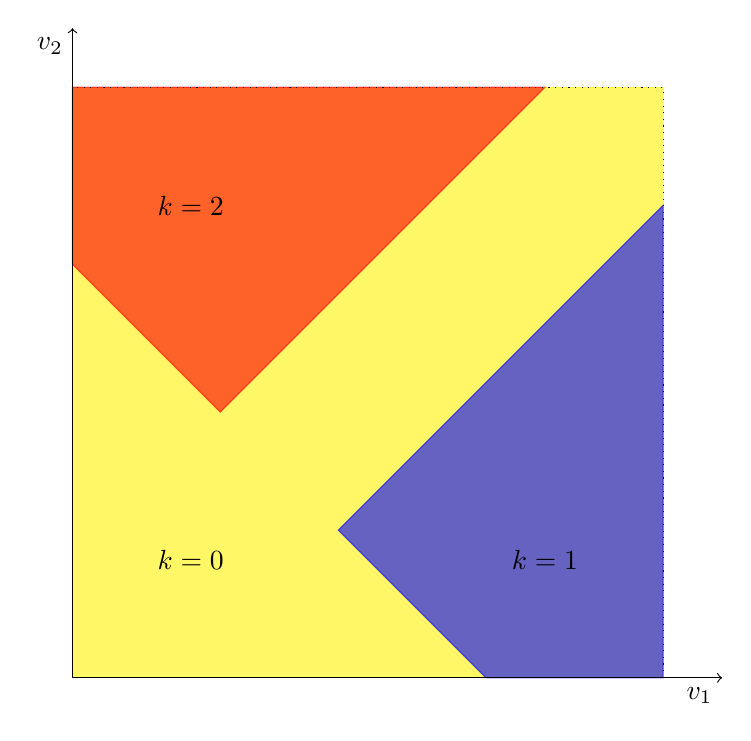
\begin{tikzpicture}[scale=7.5]
		\filldraw[yellow, opacity=0.6] (0,0) -| (1,1) -| (0,0);
		\filldraw[red, opacity=0.6] (0,0.7) -- (0.25,0.45) -- (0.8,1) -| (0,0.7);
		\filldraw[blue, opacity=0.6] (0.7,0) -- (0.45,0.25) -- (1,0.8) |- (0.7,0);
		
		\draw(0.2,0.2) node{$k=0$};
		\draw(0.2,0.8) node{$k=2$};
		\draw(0.8,0.2) node{$k=1$};
		
		% axes 
		\draw[->] (0,0) -- (1.1,0) node[below left]{$v_1$};
		\draw[->] (0,0) -- (0,1.1) node[below left]{$v_2$};
		
		% bounding box
		\draw[dotted] (1,0) |- (0,1);
		\end{tikzpicture}
		\caption{nondescript DSIC allocation} \label{fig:3}
	\end{figure}
	\fi
\end{ex}



%%------------------------------------------------------------------------------------------------


\end{document}
